\clearpage\section{Methodology}
\label{sec:sect4}
\lipsum[8]
\subsection{Subsection 4.1}
\label{subsec:subsec4.1}
\lipsum[8]
Read de book \cite{einstein} of Einstein.

\begin{figure}[H]
\label{fig:prototype1}
\centering
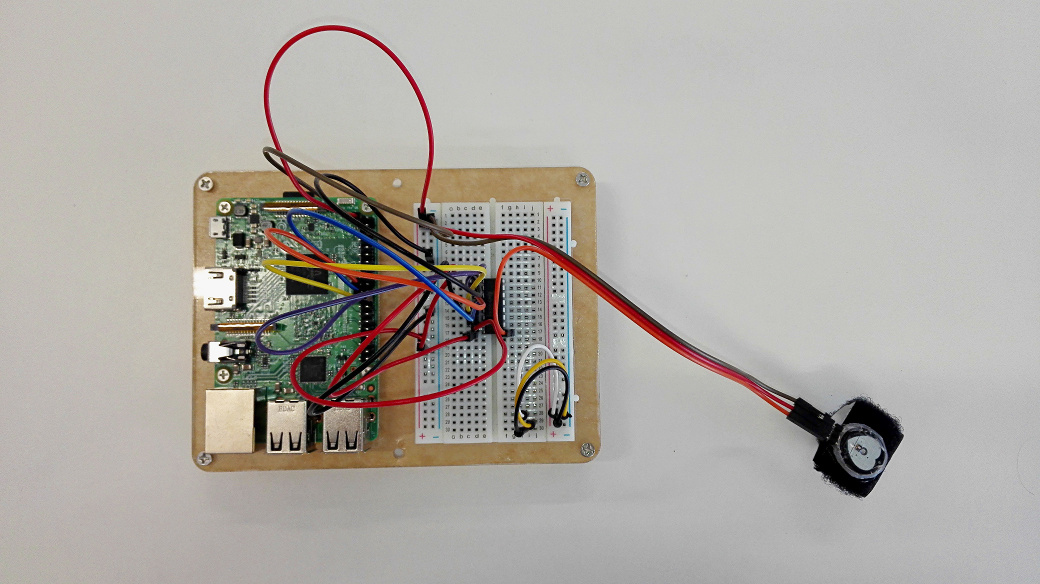
\includegraphics[width=10cm]{img/Chapter4/prototype1_edited.jpg}
\caption[Prototype setup]{\footnotesize{Prototype setup.}}
\end{figure}

\lipsum[14]

\subsection{Subsection 4.2}
\label{subsec:subsec4.2}

\begin{table}[H]
\centering
\caption[This is the caption]{ \footnotesize This is the other caption. Since the trial size of the experiments showed is one second, the number of \textit{Target} and \textit{Impostor} data corresponds to number of trials or seconds}
\label{tab:data_partition}
\footnotesize{
\begin{tabular}{@{}llcccc@{}}
\toprule
\textbf{Dataset}         & \multicolumn{1}{c}{\textbf{Label}} & \textbf{Train} & \textbf{Validation} & \textbf{Develop} & \textbf{Test} \\ \midrule
\midrule
\multirow{3}{*}{First} & Target   & $135$ & $45$  & $30$  & $30$  \\
                         & Impostor & $5,220$    & $1,740$ & $1,890$   & $2,880$    \\
\cmidrule(lr){3-5} \cmidrule(l){6-6}
                         & \#Subjects          & \multicolumn{3}{c}{$31$} & $12$ \\
\midrule
\multirow{3}{*}{Second}  & Target   & $144$ & $80$  & $48$  & $48$  \\
                         & Impostor & $2,014$    & $1,119$    & $1,343$    & $1,545$ \\
\cmidrule(lr){3-5} \cmidrule(l){6-6}
                         & \#Subjects   & \multicolumn{3}{c}{$15$} & $5$ \\ 
\bottomrule
\end{tabular}
}
\end{table}
